% This is samplepaper.tex, a sample chapter demonstrating the
% LLNCS macro package for Springer Computer Science proceedings;
% Version 2.21 of 2022/01/12
%
\documentclass[runningheads]{llncs}
%
\usepackage{changepage}
\usepackage{hyperref}
\newenvironment{myindent}{\begin{adjustwidth}{1cm}{}}{\end{adjustwidth}}

\usepackage{listings}
\usepackage{color}

\usepackage[T1]{fontenc}
% T1 fonts will be used to generate the final print and online PDFs,
% so please use T1 fonts in your manuscript whenever possible.
% Other font encondings may result in incorrect characters.
%
\usepackage{graphicx}
% Used for displaying a sample figure. If possible, figure files should
% be included in EPS format.
%
% If you use the hyperref package, please uncomment the following two lines
% to display URLs in blue roman font according to Springer's eBook style:
%\usepackage{color}
%\renewcommand\UrlFont{\color{blue}\rmfamily}
%
\begin{document}
%
\title{Formalizing the Unexpected Hanging Paradox in Coq : a New Surprise Definition} %\thanks{Supported by organization x.}}
%
%\titlerunning{Abbreviated paper title}
% If the paper title is too long for the running head, you can set
% an abbreviated paper title here
%
\author{Polina Vinogradova\inst{1}\orcidID{0000-1111-2222-3333} }
% \and
% Second Author\inst{2,3}\orcidID{1111-2222-3333-4444} \and
% Third Author\inst{3}\orcidID{2222--3333-4444-5555}}
%
\authorrunning{Polina Vinogradova}
% First names are abbreviated in the running head.
% If there are more than two authors, 'et al.' is used.
%
\institute{IOG
\email{polina.vinogradova@iohk.io}}
%
\maketitle              % typeset the header of the contribution
%
\begin{abstract}

  In this work we define a novel approach to formally specifying the
  unexpected hanging paradox, sometimes called the surprise examination paradox, using a
  constructive logical framework. We build this formal specification using the
  Coq proof assistant. This paradox requires the formalization of the notion of
  a \emph{surprise} event, which, for the purposes of this paradox, is usually interpreted as
  the inability to predict what day a specific event takes place. As in existing work,
  the use of constructive logic allows us to represent knowledge as provability.
  However, unlike many previous formalizations, we define a system,
  where intuitive conclusions can be justified formally and without inconsistency.
  We are able to achieve this by making the observation that being surprised by
  an inevitable event requires there being strictly more than one possible day on which
  it can occur. We assert that this offers a satisfying resolution to the paradox, and
  speculate that it may generalize to notions of random choice in other situations.
  We also provide a formalization of an existing interpretation of surprise,
  and an analysis of how it compares it to ours.

\keywords{surprise examination \and paradox \and unexpected hanging \and Coq \and constructive logic.}
\end{abstract}
%




\section{Introduction}

The unexpected hanging paradox, also known as the surprise examination paradox,
is a logical paradox introduced in the the Mind philosophical journal in 1948 \cite{original},
and introduced to the general public by the Scientific American Mathematical
Games column author Martin Gardner, discussed in his work \cite{diversions}.
It describes the notion of a future event that
is both certain, and not possible to predict the exact day of occurrence of,
formulated as follows :

\begin{myindent}
  A judge tells a condemned prisoner that he will be hanged at noon on one weekday
  in the following week but that the execution will be a surprise to the prisoner.
  He will not know the day of the hanging until the executioner knocks on his cell door at noon that day.

  Having reflected on his sentence, the prisoner draws the conclusion that he will
  escape from the hanging. His reasoning is in several parts. He begins by concluding
  that the "surprise hanging" can't be on Friday, as if he hasn't been hanged by
  Thursday, there is only one day left – and so it won't be a surprise if he's hanged on
  Friday. Since the judge's sentence stipulated that the hanging would be a surprise
  to him, he concludes it cannot occur on Friday.

  He then reasons that the surprise hanging cannot be on Thursday either, because
  Friday has already been eliminated and if he hasn't been hanged by Wednesday noon,
  the hanging must occur on Thursday, making a Thursday hanging not a surprise either.
  By similar reasoning, he concludes that the hanging can also not occur on Wednesday,
  Tuesday or Monday. Joyfully he retires to his cell confident that the hanging will
  not occur at all.

  The next week, the executioner knocks on the prisoner's door at noon on Wednesday –
  which, despite all the above, was an utter surprise to him. Everything the judge said came true.
\end{myindent}

Existing formalization efforts attempt to address questions like "how can we formally
define surprise?", "where is the flaw in the
reasoning of the prisoner?" and "was it contradictory for the prisoner to have been
hanged on Wednesday?". There is work on tackling these questions in multiple
different branches of philosophy and mathematics.
It appears, however, that the majority of resolutions
of this paradox reach a conclusion espousing the impossibility of
defining a consistent system with a coherent definition of surprise that is not
self contradictory.
An an extensive review of the existing approaches is given in \cite{extensivereview}.

The definition of surprise as the inability to deduce beforehand the date of the test
was first introduced in \cite{prediction}. A statistical approach to the problem
of prediction in this context is discussed in \cite{statistical}.
A proposed solution in the field of epistemology with the use of modal
logic, is presented in \cite{modalepistemic}. A an approach involving
Kripke semantics, employing the notion of persuasion, is in \cite{kripkemodal}.

The use of non-classical logic,
eg., appealing to Goedel's incompleteness, was first applied to the
paradox in \cite{goedelized}, then in \cite{godelinconsistent}, and most recently
in \cite{constructive} \cite{nonpredet}. The latter two works assume the underlying logic to itself be
constructive, as compared to reasoning via the provability operator $\mathsf{Pr}$ to indicate
a possibly non-classical statement. This approach aligns most closely with ours.

The work \cite{fourpossible} investigates the relation between the conclusions
of the non-classical logic approaches and those from epistemology, as well
as presenting four distinct approaches to formalizing the paradox, two of which
we take as the starting point for this work.

In this work, we take the point of view that the constraints of the paradox are
fixed and correctly conveyed to the prisoner. The constraints, as we formalize them,
are what is known to the prisoner on a specific day, eg. that he will be executed
by the end of the week. Like previous works cited, we chose to represent
\emph{knowledge} as constructive propositions. Whenever something is known to be
true, it is provable. When it is false, its negation is provable. Double negation
indicates that we cannot disprove a proposition, so we use this to indicate a
possibility.

Another distinction between existing work and our formalization is that
we do not use modal or temporal logic (which is the approach in \cite{modalepistemic}).
Instead, we take advantage of the expressivity of the dependent typed logic of Coq directly to
achieve the formalization of surprise at different points in time,
by parametrizing the definition of the surprise proposition
by the day about which the proposition of surprise is constructed.

Because constructive logical is notoriously slippery, we chose to use a proof
assistant (Coq, see \cite{coqmanual}) to take a closer, more high-assurance look at the
interplay between the seemingly simple conditions of this conundrum.
There is precedent for the use of proof assistants to tackle philosophical
investigation, with the most striking and recent example
being a refinement of Kant's categorical imperative upon studying its
formalization \cite{categoricalkant}.

Our definition of surprise on a day $td$ is formulated to reflect
the following natural language statement : a hanging has not occurred on or before the day $td$,
and there exist at least two distinct future days on which a hanging
is possible (ie. it is not possible to disprove that a hanging occurs on either
of those days).

We argue that this accurately represents a lack of certainty about the exact day of
the hanging, but a certainty in its inevitability, and does not contradict
the other constraints of the paradox. We do so by asking the reader to consider the following
statement : a prisoner will be hanged on Monday, but the day he will be hanged will
be a surprise. Why is this contradictory? Intuitively, it is precisely because
being surprised by an inevitable event requires there to be more than one option for
when this event may happen. This is exactly the intuition we choose to formalize here.

The crux of our paradox formalization analysis hinges on the observation that the uniqueness constraint
  is, in fact, never relevant to the formalization of the paradox --- neither in reasoning about
  any day with a possibility of future hanging (ie. on which
  a hanging has not yet happened), nor about a day on which it has already happened.
  We go on to argue that the general constraint that a hanging necessarily happens is
   also contradictory to our definition of surprise. Moreover, the looser constraint
  from previous work,
  saying that we \emph{should not be able to disprove that a hanging happens on one of the
  days} is insufficiently strong, and is implied by our definition.
  However, the intuitive conclusion normally drawn from it
  (that if a hanging is only possible Friday, it must happen then)
  is too strong, resulting in classical reasoning about surprise.

  The contributions of this paper are as follows :

  \begin{itemize}
    \item[(i)] a formal specification (in Coq) of the types and conditions of the that
    are shared among existing interpretations, using dependent types and constructive logic,
    Section \ref{sec:universal} ;
    \item[(ii)] a definition (in Coq) of surprise from a previous work, with an analysis of it
    in Section \ref{sec:one} ;
    \item[(iii)] a novel definition (in Coq) of surprise that we propose,
    Section \ref{sec:two};
    \item[(ii)] a formally verified proof that a Friday hanging is not a surprise, Section \ref{sec:two};
    \item[(iii)] a formally verified proof that our definition of
    surprise for this paradox is equivalent to the negation of the
    constraint that the hanging happens on exactly one specific day, Section \ref{sec:unique};
    \item[(iv)] an analysis of the unexpected hanging paradox offering a resolution without
    contradiction, Sections \ref{sec:two} \ref{sec:unique} \ref{sec:tgit} \ref{sec:friday};
    \item[(v)] an analysis of the relation of the informal meaning of surprise
    to its formalization.
  \end{itemize}

  For our code, see \href{https://github.com/polinavino/unexpected_hanging/blob/master/unexpected_hanging.v}.

\section{Coq and the Paradox}
\label{sec:form}

Coq is a proof assistant that offers a dependently typed formal language.
It is capable of verifying formal user-defined proofs of propositions, as well as has support
for automation of certain kinds of proofs. The choice of Coq, as opposed to another
proof assistant such as Agda, was based largely on the authors' familiarity with the system,
as any dependently typed proof verifier that supports constructive logic
would serve just as well for the purposes of this formalization.

To formalize the paradox, we need to reason about days of the week on which
the paradox could happen, so we
begin by constructing a type {\tt weekDay} the terms of which are week days :

\begin{lstlisting}
  Inductive weekDay : Type :=
    | monday : weekDay
    | tuesday : weekDay
    | wednesday : weekDay
    | thursday : weekDay
    | friday : weekDay.
\end{lstlisting}

We also define a type {\tt weekAndBefore}, which represents all the weekdays in
the type above, plus the Sunday that comes before --- the purpose of this type is to
represent all the days on which one can consider the possibility of surprise,
differentiating it from the subset of days on which the hanging can occur. We
also define the two comparison functions,

\begin{lstlisting}
  isBefore, isOnOrAfter (td : weekAndBefore) (d : weekDay) : Prop := ...
\end{lstlisting}

which compute whether a given {\tt td} is before (is on or after, respectively) {\tt d},
following real-life weekday logic, eg. Sunday is before Monday.
Both of these are classical comparisons, which we prove in our code.
From here on, we use the notation $<$ for {\tt isBefore}, and
$\geq$ for {\tt isOnOrAfter}.

We do not know what day the hanging happens on, but we can specify the type of a
function that, given a day of the week, returns $\mathsf{True}$ if we can prove the hanging
happened, and $\mathsf{False}$ if we can prove it did not. We reason about this function
in the presence of preconditions that are formal interpretations of those described
in the paradox. We leave this function as a variable :

\begin{lstlisting}[mathescape=true]
  Variable hangingOnDay : weekDay $\to$ Prop.
\end{lstlisting}

We discuss the existence of such a predicate that
works with in definition of surprise as part of future work.
Next, we define a predicate that formalizes the notion that no hanging has occurred
yet (up to and including the parameter day {\tt td}, representing \emph{today}) :

\begin{lstlisting}[mathescape=true]
  Definition noHangingYet
      (td : weekAndBefore) :=
    $\forall$ d, td $\geq$ d
    $\to$ $\neg $ hangingOnDay d.
\end{lstlisting}

This says that for any day {\tt d}, if it is before today {\tt td}, no hanging
happened on {\tt d}.

We use the double negation {\tt $\neg \neg$ hangingOnDay d} to formalize the statement that it is
not possible to disprove that a hanging occurs on day {\tt d}. That is, a hanging
is \emph{possible} on a given day.

\section{Surprise parametrization and universal conditions}
\label{sec:universal}

Notice that the {\tt noHangingYet} function we introduced is actually a
dependent proposition (a predicate), parametrized by
the day {\tt td} that is \emph{today}. This is because we are interested in
being able to reason under the conditions of the past being defined, but
would like to vary what "the past" refers to (ie. days {\tt d $\leq$ td}).

Similarly, we parametrize the
constraints of the paradox so that we are able to reason about
whether we are still within them of at each point in the week,
which is the level of detail in we are interested in. This lets us, for example,
reason about the impossibility of a surprise hanging on Friday, given that
today is Thursday, but not be able to apply the same reasoning if
today is only Wednesday, see Section \ref{sec:tgit}.

We now specify two conditions, implicit in the informal
description of the paradox :

\begin{itemize}
  \item[(i)] if today is Friday, ie. the whole
  week has passed, we know that a hanging necessarily happened
  \begin{lstlisting}[mathescape=true]
    td = someWeekDay friday
      $\to$ $\exists$ d, hangingOnDay d
  \end{lstlisting}
  \item[(ii)] if a hanging has occurred, it is unique
  \begin{lstlisting}[mathescape=true]
    ($\exists$ d, hangingOnDay d)
      $\to$ uniqueHanging dayBefore
  \end{lstlisting}
\end{itemize}

where {\tt uniqueHanging} is a predicate formalizing that after a given day {\tt td},
there can be at most one day on which a hanging occurs, and thus,
{\tt uniqueHanging dayBefore} states this about the entire week.

\begin{lstlisting}[mathescape=true]
  Definition uniqueHanging
      (td : weekAndBefore) :=
    $\forall$ d d',
    td $<$ d $\wedge$ td $<$ d' $\to$
    hangingOnDay d $\to$
    hangingOnDay d' $\to$
    d = d'.
\end{lstlisting}

We note here that the preconditions in both implications are such that if
they are satisfied, intuitively surprise should not be possible : (i)
requires that the week is already over, and (ii) requires that a hanging
has happened. The time at which we may be surprised by a hanging is strictly
before it happens and before the week is over, so neither of these should
actually play any role in the reasoning about surprise, which is reflected
in our upcoming definition of surprise. However, (i) and (ii) together express all the
other constraints of the paradox besides the one requiring the hanging to
be a surprise (now we just need to add that part!).

Surprise requires that a future hanging be possible - on more than zero
of the remaining weekdays after today.
So, the constraint that at least one future possible hanging day exists is
clearly necessary. However, the case for at least one possible day not
being sufficient to define surprise is a bit more nuanced.

\section{At least one possible day}.
\label{sec:one}

We specify this interpretation
of the conditions of the paradox for each possible day as:

\begin{lstlisting}[mathescape=true]
  Definition onePossiblePRDX (td : weekAndBefore)  :=
    (td = someWeekDay friday
      $\to$ $\exists$ d, hangingOnDay d)
    $\wedge$
    (($\exists$ d, hangingOnDay d)
      $\to$ uniqueHanging dayBefore)
    $\wedge$
    ((td $<$ friday $\wedge$ noHangingYet td) ->
      $\exists$ d, td $<$ d $\wedge$ $\neg~\neg~$ hangingOnDay d).
\end{lstlisting}

where the first two conjuncts are as described above, and
the third one corresponds to "if today is not
  yet Friday, there is a possible day on which a hanging may happen", which
  we refer to as the {\tt onePossible} definition of surprise.

This definition is one of the alternatives discussed in \cite{fourpossible}. No inconsistency
is introduced here, in fact, the hanging can still be a surprise even if it
happens on a Friday! The intuition behind this is : if no hanging happened by
Thursday, it is still only possible to prove {\tt $\neg~\neg$~hangingOnDay friday},
from which we are not able to deduce that {\tt hangingOnDay friday}.

Note here that including the constraint that \emph{a hanging must happen
by the end of the week} is still not sufficient to conclude certainty
from unique possibility. The reason for this is that the conclusion that
a hanging definitely happened on one of the week days can only be made
after Friday has come. The possibility of surprise, meanwhile, has the
precondition that the whole week has not passed yet (ie. Friday has not yet come).
These preconditions are mutually exclusive.

The condition that if a hanging has happened, it must be unique, also does not
give us any reasoning power, as we are not able to conclude {\tt hangingOnDay friday}.

Let us consider what happens if we impose an additional constraint stating that
exactly one \emph{possible} hanging
day implies that it \emph{provably happens} on a specific day. This is also explored in
\cite{fourpossible}, with a similar conclusion to the one we draw here. The following
proposition states that there is a possible hanging day, and that a possible
unique day implies certainty of hanging on that day :

\begin{lstlisting}[mathescape=true]
  Definition existsUniqueHappens :=
    ($\exists$ d, $\neg~\neg$ hangingOnDay d)
    $\wedge$
    ($\forall$ d d',
      $\neg~\neg$ hangingOnDay d
      $\to$ $\neg~\neg$ hangingOnDay d'
      $\to$ d = d')
    $\to$
    $\exists$ d, hangingOnDay d.
\end{lstlisting}

Now, the following statement expresses that {\tt existsUniqueHappens} lets us
conclude that {\tt hangingOnDay} must then be classical (the proof is in the
associated code) :

\begin{lstlisting}[mathescape=true]
  Lemma euhImpClassical :
    (uniqueHanging dayBefore) $\to$
    (exists d, $\neg~\neg~$ hangingOnDay d) $\to$
    existsUniqueHappens $\to$
    ($\forall$ d,
    $\neg~$ hangingOnDay d $\vee$ hangingOnDay d).
\end{lstlisting}

This proposition, without justification, is the crux of the reasoning the prisoner
uses to informally to arrive at the judgement that
if a hanging hasn't happened by Thursday, it must happen on Friday.
Note here that the inductive reasoning in which the prisoner engages to conclude that the
hanging cannot ever be a surprise is, in some sense, superfluous --- we can use
constructive logic reasoning to prove, without induction, that "if we can conclude
from existence plus uniqueness of a possible hanging day, that it is certain on that day,
\emph{our judgement about hanging occurring on any day must necessarily be classical}".
The proof makes use of the fact that the equality comparison {\tt d = d'} is
classical.

The intuition seems to be correct in making the assumption that a unique possibility
implies certainty, and the logic leading to this inconsistency with the informal
definition appears solid.
However, we will see that the problem lies in the attempt
to allow the possibility of, and draw conclusions from, having a \emph{unique possible }
hanging day.

This definition leaves us with the following conclusions about defining surprise as
having at least one possible hanging day :

\begin{itemize}
  \item[(i)] such a definition of surprise is not strong enough to allow us to conclude
  {\tt existsUniqueHappens}, in particular, that a hanging
  must happen Friday given that it has not occurred by Thursday, and is
  therefore not a surprise in that case ; and \newline
  \item[(ii)] if we \emph{were} to be able to conclude {\tt existsUniqueHappens},
  reasoning about surprise
  becomes classical, so we can always figure out the hanging day in advance.
\end{itemize}

Both possibilities appear problematic : (i) does not allow us to make
a conclusion that we would like make,
and (ii) does not support reasoning non-classically, which removes any ambiguity
about the future hanging day, and therefore, the possibility of surprise.
Let us see why adding a different additional constraint (ie. other than deriving
certainty from a unique possibility) will help.

\section{Full paradox : at least two possible days}.
\label{sec:two}

The way we propose to strengthen the conditions of surprise is by increasing
the number of possible days required for surprise to two :

\begin{lstlisting}[mathescape=true]
  Definition twoPossible
      (td : weekAndBefore) :=
    $\exists$ d d', d $\neq$ d'
    $\wedge$ $\neg \neg$ hangingOnDay d
    $\wedge$ $\neg \neg$ hangingOnDay d'
    $\wedge$ td $<$ d $\wedge$ td $<$ d'.
\end{lstlisting}

We can read this as follows :

\begin{myindent}
  There exist two distinct days after the day {\tt td} such that
  a hanging is possible (ie. cannot disprove that it happens then)
\end{myindent}

Intuitively, this constraint makes sense --- if I am not sure what day something
will occur, there must be at least two possible future days on which it could occur,
as expressed in {\tt twoPossible}.
To formulate the complete conditions of the paradox for each day, we formalize that, in addition
to the two constraints justified earlier, we include the constraint that
"if today is before Friday, and no hanging has yet happened, there are at least
two possible distinct hanging days in the future" :

\begin{lstlisting}[mathescape=true]
  Definition twoPossiblePRDX
      (td : weekAndBefore)  :=
    (td = someWeekDay friday
      $\to$ $\exists$ d, hangingOnDay d)
    $\wedge$
    (($\exists$ d, hangingOnDay d)
      $\to$ uniqueHanging dayBefore)
    $\wedge$
    ((td $<$ friday $\wedge$ noHangingYet td) $\to$
      twoPossible td).
\end{lstlisting}

Now, the first thing we can formally conclude about this definition is that it indeed rules out
a Friday hanging. The following lemma says that it is not possible that by Thursday,
no hanging has happened, but there are still two distinct possible days for it to
happen in the future.

\begin{lstlisting}[mathescape=true]
  Lemma cantBeSurpFriday :
    twoPossiblePRDX (someWeekDay thursday)
    $\to$ noHangingYet (someWeekDay thursday)
    $\to$ False.
\end{lstlisting}

The proof (see code) is trivial, since there is only one day (Friday) left in the week,
and no hangings are possible on past days.

This reasoning does not work, however, for any
day before Thursday, since there are (for any day before Thursday) at least two future
days about which we have no
data contradicting the possibility of a hanging.
Inductive reasoning in attempt to conclude that a Thursday hanging is
predictable on Wednesday does not work because we do not have enough data on Wednesday
to conclude whether a hanging will be Thursday or Friday. That is, to discount Friday
as a possibility of surprise hanging, we \emph{need to know that there was no
hanging Thursday}.

So, this definition of surprise aligns with our intuition by making surprise
by a Friday hanging possible, but does not appear to contradict the possibility
on any other day. It has, however, an unintuitive feature.

\section{Negation of uniqueness. }
\label{sec:unique}

With this definition of surprise, surprise is never possible when there is
exactly one possible hanging day. The constraint, {\tt uniqueHanging}, that
a (provable) hanging day is unique is, in fact, equivalent to the constraint
that the (possible) hanging day must be unique,

\begin{lstlisting}[mathescape=true]
  Definition uniqueMaybe
      (td : weekAndBefore) :=
    $\forall$ d d',
    td $<$ d $\wedge$ td $<$ d' $\to$
    $\neg~\neg$ hangingOnDay d $\to$
    $\neg~\neg$ hangingOnDay d' $\to$
    d = d'.
\end{lstlisting}

We parametrize the above propositions by $td$ to express that they apply to
a specific subset of the week days --- those days that are after today,
eg., {\tt uniqueMaybe dayBefore} specifies that if a hanging is provable to be
on \emph{any two weekdays}, those days must be the same.
We prove that they the two propositions are equivalent :

\begin{lstlisting}[mathescape=true]
  Lemma uniqueMaybeEqv
      (td : weekAndBefore) :
    uniqueHanging td
    $\leftrightarrow$
    uniqueMaybe td.
\end{lstlisting}

The proof of this relies on, again, the fact that $d = d'$ is a classical
comparison. Moreover, the {\tt twoPossible} constraint
in our definition of surprise \emph{implies the negation of} {\tt uniqueHanging}
(and therefore also {\tt uniqueMaybe}) :

\begin{lstlisting}[mathescape=true]
  Lemma twoNotUnique :
    $\forall$ td,
    twoPossible td $\to$
    $\neg$ uniqueHanging td.
\end{lstlisting}

We make an observations about this : a future possible day of the hanging is
necessarily not unique. This seems wrong --- we would expect a hanging to be
unique, it's implicit in the
description of the paradox. Let us inspect this closer, however.
Our conditions of this paradox on day $td$ are that either
the week is over and the hanging has occurred, or, for $td \neq thrusday, friday$ surprise is
only possible if the hanging has not yet happened. We not that

Once a hanging occurs, we can no longer reason about it having been a surprise
That is, a judgement of surprise can only made about
an event in the context of a lack of information about it (in this case,
whether a hanging will happen on a specific future day).

This is perhaps the most paradoxical idea here. Any reasoning that includes
in its hypotheses both that a hanging happened after {\tt td} and that it is a surprise
(in our case, specified as {\tt twoPossible td}) is intuitively meaningless. This is not a
formal statement, but rather a statement about what surprise means. You cannot
be surprised by an event that has already occurred.

As an aside, this is a nuance of how we use language. One can reason about a surprising past
event from the perspective of a time prior to that event, but to do so,
the available hypotheses must only include information known at that time, ie.
not the occurrence of that event. This is why statements such as "I was surprised
by a hanging when it happened", or "last week I was surprised when I found out
that it had happened to my friend two weeks ago", make sense, and are usually
what is meant when one says "I am surprised by a past hanging".

Now, back to why it is ok for hanging day to not to be required to be unique
before the hanging occurs : once the (first) hanging
occurs on some {\tt d}, we now have {\tt $\neg~$ noHangingYet (someWeekDay d)}.
That means that the {\tt twoPossible (someWeekDay d)} implication of {\tt noHangingYet (someWeekDay d)}
is no longer required to hold, and also that {\tt exists d, hangingOnDay d}, so
its consequence {\tt uniqueHanging dayBefore} is now required to hold.
So, uniqueness constraint "kicks in" after the hanging first happens.

\section{TGI Thursday}
\label{sec:tgit}

With this definition of the paradox, surprise is already not possible on Thursday.
The reason for this is not that the definition allows us to conclude that a hanging will
definitely happen on Friday once we get to Thursday. Rather, it is that the
conditions for surprise are not satisfied on Thursday in another way (a missing
a possible day).

We have already discussed that, since the definition
is parametrized by the day on which we judge whether the paradox conditions
are met, surprise (and all other conditions of the paradox) actually form
a different proposition for each day. And so, an impossibility of surprise
Thursday does not affect what we can prove about the rest of the days.
With that in mind, we can choose to make a special case
for the paradox characterization, which only applies when exactly one day remains as a possibility
for a hanging --- and there is only one such day, Thursday.

The special case to add is exactly the conclusion we rejected in the {\tt onePossible}
version of surprise : {\tt existsUniqueHappens}. Note here that
the difference between one- and two-possible versions of surprise, with respect
to adding this constraint,
is that in the two-case, we use the paradox definition to conclude that Thursday
does not allow surprise. In the one-case, on the other hand, we \emph{rely} on the reasoning in
{\tt existsUniqueHappens} to conclude surprise is not possible on Thursday,
which leads an unsavoury conclusion.

We do not add it, after all, even though the reasoning it allows us to do
appears coherent. The reason for this is that the preconditions of this
constraint already conflict with those of the {\tt twoPossible} surprise definition, as well
as with the preconditions of the universal paradox constraints. So, it does not
add additional reasoning power to our definition.

\section{The week is done }
\label{sec:friday}

In both versions of the definition of surprise ({\tt twoPossiblePRDX} and
{\tt onePossiblePRDX}), Friday is explicitly excluded from the surprise
part of the paradox definition.
We exclude this day since Friday arriving means that the
week has passed and there is no possible way for a hanging to occur. We also
conclude that the hanging must have already occurred.

\section{Conclusion and Future Work}

We have presented a formalization of the unexpected hanging paradox that appears to capture the
conditions of the paradox, meanwhile both aligning with the
intuition about Friday, and not reasoning ourselves out of the hanging entirely.
We formalized this definition, along with some related proofs, in the Coq
proof assistant.
A few key ideas were needed to achieve this.

The starting point was the observation that constructive logic
is required to represent knowledge in order to allow for the possibility that we
may not know something to be either true or false --- such as whether a hanging
occured on a given day. Next, we observe that surprise is a different notion
on each of the days, so our definition is parametrized by the day on which
we reason about its possibility. Then, we notice that the universal conditions of the
paradox only apply when surprise is intuitively not possible (ie. the end of the
week or after the hanging), and we separate these out from the surprise specification.

Finally, we formalize and compare two definitions of surprise. The first,
{\tt onePossible}, has been explored in prior work. We discuss why it has
consequences contradictory to our intuition about the paradox, and attempts to
rectify them in the intuitive way result in the
exact undesirable conclusion that the prisoner makes in the paradox description.
The second is {\tt twoPossible}, which we proposed, and it is a strengthening of
the first definition that does not cause the reasoning about the future hanging to
become classical (unlike {\tt onePossible}).

The surprise formalization we propose drops (in fact, negates) the constraint
guaranteeing the uniqueness of the future hanging. The subtlety here is in the idea that the
constraint still applies \emph{once the hanging happens}, but multiple
distinct days for a future hanging are still required up until then.
Our Coq formalization of the paradox stands out from existing work in (i)
its mechanization of the problem (ii) providing a resolution to the paradox that aligns with
intuition (iii) leading us to making new subtle observations about the
constraints of the problem and how they are hidden by language.

As part of future work, we would like to show that for each day  {\tt td}, there
is a function {\tt hangingOn}, that assigns to each day proposition values about the
occurrence of the hanging on that day, such that
for each day except Thursday, the conditions of the paradox are satisfied by this
function.

\begin{lstlisting}[mathescape=true]
  Proposition existsHangFunc td :
    $\exists$ hangingOn,
    td $\neq$ (someWeekDay thursday) $\to$
    twoPossiblePRDX_param hangingOn td.
\end{lstlisting}

Note here that there is no one function that makes the assignment for all days
{\tt td}. The reason for this is that depending on the week day, these must be different.
For example, on Friday, a unique hanging must have been assigned, which contradicts
the two necessary possibilities that must exist for other week days. In fact,
we would even be able to define a function of type

{\tt todayIsAndHangingOn : weekAndBefore $\to$ weekDay $\to$ Prop}

which returns a proposition about whether a hanging has happened on not on a given day {\tt d}, such that
it is in accordance with the rules of the paradox as they apply to a specific
{\tt td}.

Proving the above proposition would valuable in
establishing our formalization as the universally accepted one. Additionally,
this paradox formalization could be further analyzed by way of considering its
relationship to the axiom of choice. This is due to its (at least surface level)
resemblance to the way the AC makes a connection between classical logic
and a choice function \cite{accomp} as well as arbitrary elements \cite{randomness}.

Another future direction we consider is generalizing the surprise hanging
approach we propose to using constructive logic for describing and proving
the existence of a function {\tt myPick}
which represents choosing an arbitrary value from a decidable set. In particular,
given a decidable set {\tt W}, \newline

\begin{myindent}
For any subset {\tt S $\subseteq$ W} of cardinality at least 2, such that for all
{\tt s $\in$ W - S}, $\neg ${\tt myPick s}, there exist at least two distinct
elements in {\tt S}, such that $\neg~\neg~${\tt myPick s}.
\end{myindent}

% \section{First Section}
% \subsection{A Subsection Sample}
% Please note that the first paragraph of a section or subsection is
% not indented. The first paragraph that follows a table, figure,
% equation etc. does not need an indent, either.
%
% Subsequent paragraphs, however, are indented.
%
% \subsubsection{Sample Heading (Third Level)} Only two levels of
% headings should be numbered. Lower level headings remain unnumbered;
% they are formatted as run-in headings.
%
% \paragraph{Sample Heading (Fourth Level)}
% The contribution should contain no more than four levels of
% headings. Table~\ref{tab1} gives a summary of all heading levels.
%
% \begin{table}
% \caption{Table captions should be placed above the
% tables.}\label{tab1}
% \begin{tabular}{|l|l|l|}
% \hline
% Heading level &  Example & Font size and style\\
% \hline
% Title (centered) &  {\Large\bfseries Lecture Notes} & 14 point, bold\\
% 1st-level heading &  {\large\bfseries 1 Introduction} & 12 point, bold\\
% 2nd-level heading & {\bfseries 2.1 Printing Area} & 10 point, bold\\
% 3rd-level heading & {\bfseries Run-in Heading in Bold.} Text follows & 10 point, bold\\
% 4th-level heading & {\itshape Lowest Level Heading.} Text follows & 10 point, italic\\
% \hline
% \end{tabular}
% \end{table}
%
%
% \noindent Displayed equations are centered and set on a separate
% line.
% \begin{equation}
% x + y = z
% \end{equation}
% Please try to avoid rasterized images for line-art diagrams and
% schemas. Whenever possible, use vector graphics instead (see
% Fig.~\ref{fig1}).
%
% \begin{figure}
% 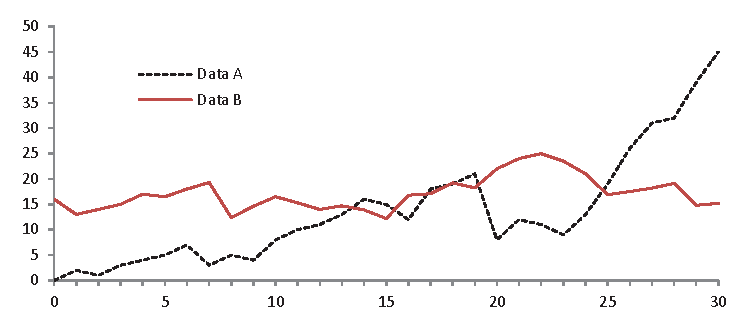
\includegraphics[width=\textwidth]{fig1.eps}
% \caption{A figure caption is always placed below the illustration.
% Please note that short captions are centered, while long ones are
% justified by the macro package automatically.} \label{fig1}
% \end{figure}
%
% \begin{theorem}
% This is a sample theorem. The run-in heading is set in bold, while
% the following text appears in italics. Definitions, lemmas,
% propositions, and corollaries are styled the same way.
% \end{theorem}
% %
% % the environments 'definition', 'lemma', 'proposition', 'corollary',
% % 'remark', and 'example' are defined in the LLNCS documentclass as well.
% %
% \begin{proof}
% Proofs, examples, and remarks have the initial word in italics,
% while the following text appears in normal font.
% \end{proof}
% For citations of references, we prefer the use of square brackets
% and consecutive numbers. Citations using labels or the author/year
% convention are also acceptable. The following bibliography provides
% a sample reference list with entries for journal
% articles~\cite{ref_article1}, an LNCS chapter~\cite{ref_lncs1}, a
% book~\cite{ref_book1}, proceedings without editors~\cite{ref_proc1},
% and a homepage~\cite{ref_url1}. Multiple citations are grouped
% \cite{ref_article1,ref_lncs1,ref_book1},
% \cite{ref_article1,ref_book1,ref_proc1,ref_url1}.

\subsubsection{Acknowledgements} Please place your acknowledgments at
the end of the paper, preceded by an unnumbered run-in heading (i.e.
3rd-level heading).


---- Bibliography ----

BibTeX users should specify bibliography style 'splncs04'.
References will then be sorted and formatted in the correct style.

\bibliographystyle{splncs04}
\bibliography{hanging-bib}


\end{document}
